\begin{figure}
  \centering
  \begin{tabular}{ccc}
    \begin{minipage}{0.330\hsize}
      \centering
      $\pi^-\Sigma^+$ mode
      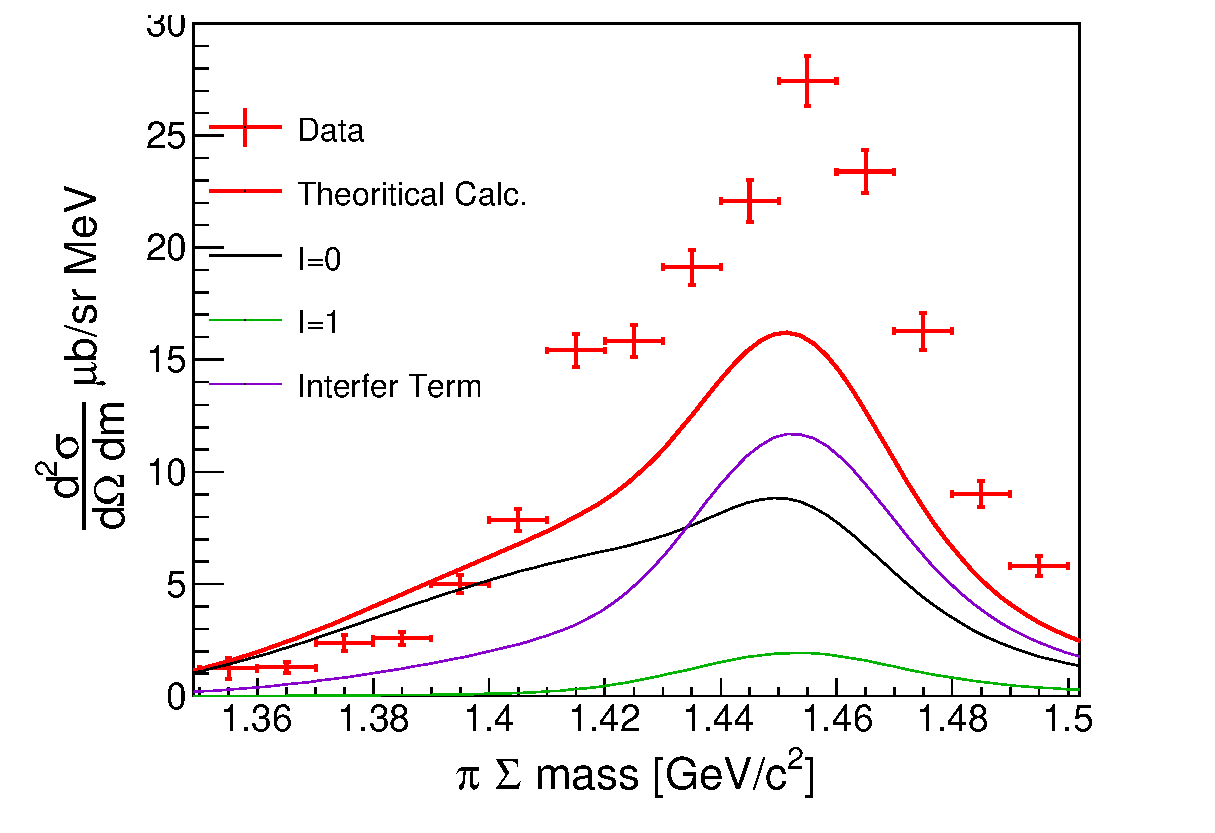
\includegraphics[width=4.5cm]{../pic/Dron/fit_model_A_fix_Phi/pimSp_fit.eps}
    \end{minipage}

    \begin{minipage}{0.33\hsize}
      \centering
      $\pi^+\Sigma^-$ mode
      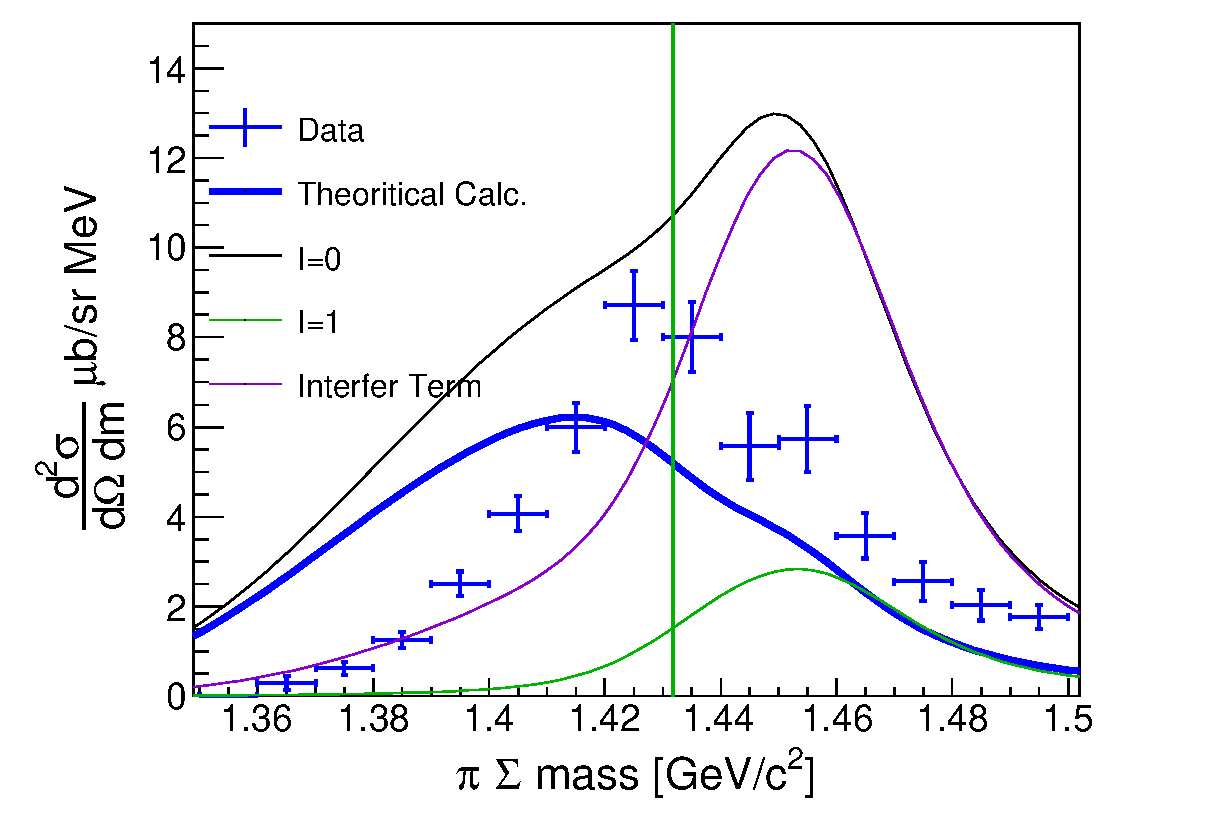
\includegraphics[width=4.5cm]{../pic/Dron/fit_model_A_fix_Phi/pipSm_fit.eps}
    \end{minipage}

    \begin{minipage}{0.33\hsize}
      \centering
      $\pi^-\Sigma^0$ mode
      \includegraphics[width=4.5cm]{../pic/Dron/fit_model_A_fix_Phi/pimS0_fit.eps}
    \end{minipage}
  \end{tabular}

  \begin{tabular}{cc}
    \begin{minipage}{0.5\hsize}
      \centering
      $I=0$\\
      \includegraphics[width=4.5cm]{../pic/Dron/fit_model_A_fix_Phi/I0_fit.eps}
    \end{minipage}
    
    \begin{minipage}{0.5\hsize}
      \centering
      Interfer\\
      \includegraphics[width=4.5cm]{../pic/Dron/fit_model_A_fix_Phi/interfer_fit.eps}
    \end{minipage}
  \end{tabular}
  \caption{
    These figures show fitting result about $A_{I=0}$ and $A_{I=1}$ using model.A.
    Above figures are used fitting.
    Left, center and right represents $\pi^-\Sigma^+$, $\pi^+\Sigma^-$ and pure $I=1$ $\pi^-\Sigma^0$ channels.
    Bottom figures show calculated components.
    Left and right indicate $I=0$ and $I=0$ and $I=1$ interference. (Pure $I=1$ corespond to $\pi^-\Sigma^0$(top right))
  }
  \label{fig:fit_A_scale}
\end{figure}
